
\documentclass[12pt]{book}

\usepackage [spanish] {babel}
\usepackage [T1]{fontenc}
\usepackage [utf8]{inputenc}
\usepackage {graphicx}
\usepackage{anysize} 
\usepackage[bookmarks=true]{hyperref}
\usepackage{bm} 
%\usepackage{natbib}
\usepackage{color}

\marginsize{4cm}{3cm}{3cm}{4cm}
\usepackage{times}

%No indent document
\setlength\parindent{0pt}

%MY COMMANDS
\definecolor{gray}{rgb}{0.5,0.5,0.2}
\newcommand{\colored}[1]{\textcolor{gray}{\bf #1}}

\newcommand{\bds}[1]{\boldsymbol{ #1 }}
\newcommand{\sub}[1]{\mbox{\scriptsize{#1}}}
\newcommand{\der}[2]{ \frac{ \partial #1 }{\partial #2} }
\newcommand{\dtot}[2]{ \frac{ d #1 }{d #2} }
\newcommand{\pr}[1]{ \left( #1 \right) }
\newcommand{\cor}[1]{ \left[ #1 \right] }
\newcommand{\lla}[1]{ \left\{ #1 \right\} }
\newcommand{\eq}[2]{\begin{equation} \label{#1} #2 \end{equation}}

%CODE COMMANDS============================================================
\newcommand{\python}{\textit{Python} }
\newcommand{\ipython}{\textit{iPython} }
\newcommand{\numpy}{\textit{NumPy} }
\newcommand{\scipy}{\textit{SciPy} }
\newcommand{\matplotlib}{\textit{Matplotlib} }
\newcommand{\mayavi}{\textit{MayaVi2} }
\newcommand{\tkinter}{\textit{TKinter} }

\usepackage{color}
\definecolor{gray97}{gray}{.97}
\definecolor{gray75}{gray}{.75}
\definecolor{gray45}{gray}{.45}

\usepackage{listings}
\lstset{ frame=Ltb,
framerule=0pt,
aboveskip=0.5cm,
framextopmargin=3pt,
framexbottommargin=3pt,
framexleftmargin=0.4cm,
framesep=0pt,
rulesep=.4pt,
backgroundcolor=\color{gray97},
rulesepcolor=\color{black},
%
stringstyle=\ttfamily,
showstringspaces = false,
basicstyle=\small\ttfamily,
commentstyle=\color{gray45},
keywordstyle=\bfseries,
%
numbers=left,
numbersep=15pt,
numberstyle=\tiny,
numberfirstline = false,
breaklines=true,
}

% minimizar fragmentado de listados
\lstnewenvironment{listing}[1][]
{\lstset{#1}\pagebreak[0]}{\pagebreak[0]}

\lstdefinestyle{consola}
{basicstyle=\scriptsize\bf\ttfamily,
backgroundcolor=\color{gray75},
}

\lstdefinestyle{python}
{language=python,
}
%=========================================================================

%#########################################################################
%	FRONT PAGE
%#########################################################################
\begin{document}
\title{Suplemento Computacional \\
\begin{Huge}
\textbf{Electricidad y Magnetismo}
\end{Huge}}
\author{ Sebastian Bustamante Jaramillo\\ \begin{small}
macsebas33@gmail.com
\end{small} \\ \vspace{5cm} \\
\includegraphics[width=3cm]{pictures/UdeA_Shield} \\
Facultad de Ciencias Exactas y Naturales \\ 
Universidad de Antioquia }
\date{}
\maketitle
%#########################################################################



%#########################################################################
%	TABLE OF CONTENTS
%#########################################################################
\newpage{\pagestyle{empty}\cleardoublepage}  

\tableofcontents
\newpage{\pagestyle{empty}\cleardoublepage}  
%#########################################################################



%#########################################################################
%	INTRODUCTION
%#########################################################################

\include{chapters/introduction}

%#########################################################################



%#########################################################################
%	1. ELECTROSTATIC
%#########################################################################

\include{chapters/electrostatic}

%#########################################################################





%#########################################################################
%	2. MAGNETOESTATIC
%#########################################################################

%#########################################################################
\chapter{Magnetostática}
\label{cha:magnetostatic}

%#########################################################################


%*************************************************************************
\section{Ejercicios}
\label{sec:ejercicios}

\
\subsection*{Ejercicio 1 \large{$\pr{\star}$}}

\textbf{Trayectoria en campo no homogéneo}

Considere una partícula de masa $m$ y carga $q$ embebida en un campo 
magnético con la siguiente forma funcional.

\[ \bds B(x, y) = A(x^2+y^2)\bds k \]

Haga un código que utilice la rutina de integración \texttt{RungeKutta4.py} 
de la demostración \ref{sec:DEMO2_03} para integrar la trayectoria de esta 
partícula en el campo $\bds B$. Puede guiarse de la demostración 
\ref{sec:DEMO2_03}, además puede usar valores numéricos de las condiciones 
iniciales, constante $A$, masa $m$ y carga $q$ de su elección.
Finalmente grafique la trayectoria calculada de la partícula cargada y 
realice una animación 3D de la partícula usando la libreria \mayavi.

\textit{Hint:} En la ventana de animación, es conveniente crear una mesa 
con el fin de tener un punto de referencia para notar el movimiento de la 
partícula.

\

\subsection*{Ejercicio 2 \large{$\pr{\star}$}}

\textbf{Billar electrostático con campo magnético}


Considere la demostración \ref{sec:DEMO2_03}. Modifique ambos scripts para
incluir la acción de un campo magnético uniforme y homogéneo que entra hacia
el tablero. La magnitud del campo magnético es de libre elección.


\subsection*{Ejercicio 3 \large{$\pr{\star}$}}

\textbf{Campo magnético de 4 corrientes}

Considere cuatro alambres por los cuales circula una corriente $I_0$, tal
como se muestra en la siguiente figura. Usando la función \texttt{quiver}
de \matplotlib, graficar las líneas de campo magnético en un plano 
perpendicular a las corrientes. Escoja los valores que desee para las 
cantidades del problema.

%.........................................................................
%Charged bar
\begin{figure}[htbp]
	\centering
	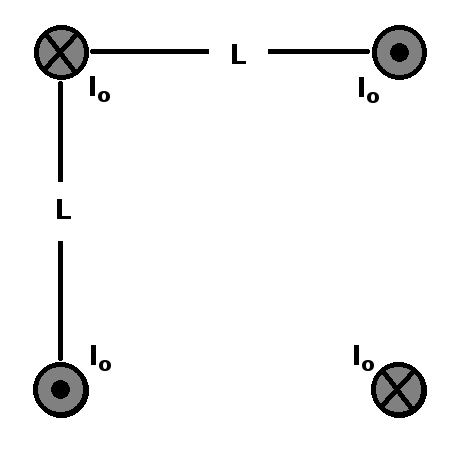
\includegraphics[width=0.4
	\textwidth]
	{./pictures/fourcorrients.png}

	\caption{\small{Cuatro corrientes de igual magnitud.}}
	
	\label{fig:fourcorrients}
\end{figure}
%.........................................................................


\subsection*{Ejercicio 4 \large{$\pr{\star \star}$}}

\textbf{Partícula en un campo dipolar}

Considere una particula cargada en un campo magnetico dipolar, integre 
numéricamente usando la rutina de integración \texttt{RungeKutta4.py} la 
trayectoria de la partícula. Realice los siguiente numerales

\
\begin{itemize}
\item [\textbf{a)}] Grafique usando la función \texttt{quiver} de \matplotlib las 
líneas de campo magnético.
\item [\textbf{b)}] Encuentre una condición inicial (velocidad y posición) para
la cual la partícula interactúe apreciablemente con el campo magnético.
Una interacción interesante puede ser el confinamiento de la trayectoria en
zonas cercanas a los polos del dipolo (Este fenómeno explica las auroras 
boreales). Guarde la trayectoria obtenida en un archivo de texto con el formato
\texttt{[x, y, z, vx, vy, vz]}.  
\item[\textbf{c)}] Realice una animación 3D usando \mayavi donde ilustre el 
movimiento de la partícula cargada.

\textit{Hint:} En la ventana de animación, es conveniente crear un objeto
con el fin de tener un punto de referencia para notar el movimiento de la 
partícula. Este objeto puede ser una esfera en el centro del campo dipolar.

\end{itemize}

Escoja los valores que desee para las cantidades físicas del problema.

%*************************************************************************

%#########################################################################

\begin{thebibliography}{}
\bibitem[1]{purcell} Purcell E. M. Electricity and Magnetism, Berkeley 
Physics Course Vol. 2. Mc Graw Hill. 1965. 
\bibitem[2]{finn} Alonso \& Finn. Física, Campos y Ondas Vol. 2. Addison-Wesley. 
1998.
\bibitem[3]{sears} Sears, Zemanski, Young \& Freedman, Física Universitaria Vol. 2. 
Pearson Addison-Wesley, 11 ed, 2004.
\end{thebibliography}

\end{document}